\chapter{Strongly Connected Directed Graphs}
Rishnak wanted to continue his discussion with Ajur on the topic of directed graphs\footnote{Sometimes directed graphs are called \textit{digraphs}} and caught up with Ajur and Jura.

Rishnak asked Ajur if he remembered what relations were.

Ajur said, ``I think so, yes. A relation describes how two things interact with one another, so a relation could be symmetric like a friendship---if person~A is a friend of person~B, then person~B is also a friend of person~A. This would be an undirected graph.''

Rishnak nodded and said, ``Right, and a relation can also be asymmetric, like a follower on social media---if person~A follows the feed of person~B, it might not be the case that person~B follows person~A---and this would be a directed graph. There are many relations that are asymmetric, for example less than or precedence relations, as well as parent or winner relations. In each case, we can model the asymmetric relation as a directed graph.''

Ajur nodded, understanding thus far.

Rishnak continued, ``Similar to a path or a walk in an undirected graph, we can also define a path or a walk in directed graph. Remember an undirected graph is connected if there is a path between every pair of vertices. A directed graph is said to be \textit{strongly connected} if there is directed path between every pair of vertices. Here''---Rishnak flashed his hands and a graph appeared [Figure~\ref{15g1}]---``look at this graph.''

\begin{figure}
\begin{center}
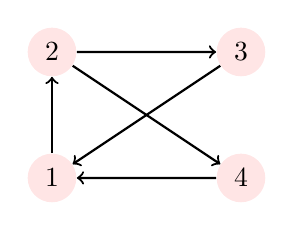
\begin{tikzpicture}
  [scale=.8,auto=left,every node/.style={circle,fill=red!10}]
  \node (n1) at (1,7) {1};
  \node (n2) at (1,9)  {2};
  \node (n3) at (4,9)  {3};
  \node (n4) at (4,7) {4};
 \path[->, draw,thick] 
        (n1) edge (n2)
         (n3) edge (n1)
        (n2) edge (n3)
        (n2) edge (n4)
        (n4) edge  (n1);

\end{tikzpicture}
\caption{Strongly connected directed graph for which there is a path between every pair of vertices}\label{15g1}
\end{center}
\end{figure}

Ajur said, ``From any vertex, we can follow one or more directed edges to get to any other vertex in the graph.''

Rishnak said, ``Exactly. Can you construct a directed graph with four vertices that is strongly connected with a minimal number of edges?''

Ajur thought for a moment, grabbed a stick, and drew a graph in the dirt [Figure~\ref{15g2}]. He said, ``Sure, this graph is strongly connected with only four edges.''

\begin{figure}
\begin{center}
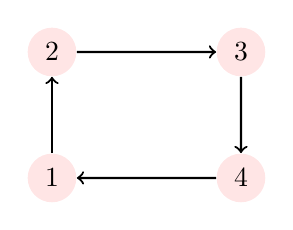
\begin{tikzpicture}
  [scale=.8,auto=left,every node/.style={circle,fill=red!10}]
  \node (n1) at (1,7) {1};
  \node (n2) at (1,9)  {2};
  \node (n3) at (4,9)  {3};
  \node (n4) at (4,7) {4};
 \path[->, draw,thick] 
         (n1) edge (n2)
        (n2) edge (n3)
        (n3) edge (n4)
        (n4) edge  (n1);

\end{tikzpicture}
\caption{Strongly connected directed graph with a minimal number of edges for which there is a path between every pair of vertices}\label{15g2}
\end{center}
\end{figure}

Pleased, Rishnak said, ``Precisely. A strongly connected directed graph must have at least~$n$ edges, but we can have a directed graph that is not strongly connected even with~$\frac{1}{2}n(n-1)$ edges.''---Rishnak waved his hands and a new graph appeared [Figure~\ref{15g3}]---``How many edges do we need to add to this graph to make it strongly connected?''

\begin{figure}
\begin{center}
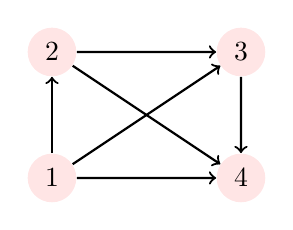
\begin{tikzpicture}
  [scale=.8,auto=left,every node/.style={circle,fill=red!10}]
  \node (n1) at (1,7) {1};
  \node (n2) at (1,9)  {2};
  \node (n3) at (4,9)  {3};
  \node (n4) at (4,7) {4};
 \path[->, draw,thick] 
        (n1) edge (n2)
         (n1) edge (n3)
        (n2) edge (n3)
        (n2) edge (n4)
        (n3) edge (n4)
        (n1) edge  (n4);

\end{tikzpicture}
\caption{A directed graph that is not strongly connected}\label{15g3}
\end{center}
\end{figure}

Ajur thought for a minute, then said, ``Just one edge. If we add an edge from vertex~4 to vertex~1, then the directed graph would become strongly connected since we could get from any vertex to any other vertex.''

Rishnak smiled. Probing further, he asked, ``In this first graph [Figure~\ref{15g1}], how many edges must we remove to make it not strongly connected?''

Ajur quickly said, ``Again just one edge. If the edge from vertex~1 to vertex~2 was removed, then the directed graph would no longer be strongly connected since no vertex is reachable from vertex~1.''

Rishnak's smile broadened. He said, ``Good. This is an important concept to master, since edge removal problems relate to edge failures in a wide variety of problems that we can model using graphs.''

Rishnak paused for a moment, then said, ``The \textit{transitive closure} of directed graph~$G=(V,E)$ is directed graph~$H=(V,E_1)$ such that there is a directed edge in~$H$ between two vertices~$u$ and~$v$ if there is a directed path from vertex~$u$ to vertex~$v$ in~$G$.''

Ajur could not contain his excitement as he said, ``I see. And the transitive closure of a strongly connected graph will always be a complete directed graph. Let me draw the graph.''---Ajur hurriedly drew a new graph in the dirt [Figure~\ref{15g4}]---``Here is the transitive closure of both of the graphs you have shown me.''

Rishnak said, ``And how do you reason that?''

Ajur said, ``Two key points:
\begin{enumerate}
    \item In the original directed graph, there is a directed path between every pair of vertices. We know this because the graph is strongly connected.
    \item In the transitive closure graph, there is an edge between every pair of vertices since there is a path between every pair of vertices in the original graph.''
\end{enumerate}

\begin{figure}
\begin{center}
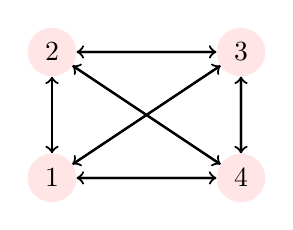
\begin{tikzpicture}
  [scale=.8,auto=left,every node/.style={circle,fill=red!10}]
  \node (n1) at (1,7) {1};
  \node (n2) at (1,9)  {2};
  \node (n3) at (4,9)  {3};
  \node (n4) at (4,7) {4};
 \path[->, draw,thick] 
         (n1) edge (n2)
         (n2) edge (n1)
        (n2) edge (n3)
        (n3) edge (n2)
        (n3) edge (n4)
        (n4) edge (n3)
        (n1) edge (n4)
        (n1) edge (n3)
        (n3) edge (n1)
        (n2) edge (n4)
        (n4) edge (n2)
        (n4) edge  (n1);

\end{tikzpicture}
\caption{The transitive closure of the directed graphs shown in Figure~\ref{15g1} and Figure~\ref{15g2}}\label{15g4}
\end{center}
\end{figure}

Rishnak nodded.

Ajur continued, ``For example, on a social media page, if I post a message, it's visible to my friends. And if my friends share that post, then that post will become visible to all friends of that friend. That's how transitive closure works. If someone posts a message, it quickly will be seen
by almost everyone!''

Rishnak smiled and said, ``Yes, exactly. Here is a similar problem, this one from one of my favorite books by Henry Ernest Dudeney.\footnote{The book is ``536 Puzzles and Curious Problems.''} Problem~452 states that we have four teams, Scotland, England, Wales, and Ireland. This table of data''---Rishnak flashed his hands and the data appeared in front of Ajur [Table~\ref{15t1}]---``shows the results of their football matches, well soccer I mean. Can you model this problem using a directed graph?''

\begin{table}
\begin{center}
\begin{tabular}{ |p{3cm}||p{1.5cm}||p{1.5cm}||p{1.5cm}||p{1.5cm}||  }
 \hline
 \multicolumn{5}{|c|}{Game Results} \\
 \hline
 Country Name & Played & Won & Lost & Drawn \\
 \hline
 Scotland & 3 & 3 & 0 & 0 \\
 England  & 3 & 1 & 1 & 1 \\
 Wales    & 3 & 1 & 1 & 1 \\
 Ireland  & 3 & 0 & 3 & 0 \\
  \hline
\end{tabular}
\caption{Results of six football (soccer) matches}\label{15t1}
\end{center}
\end{table}

Ajur thought for a bit and was able to draw a directed graph corresponding to this table [Figure~\ref{15g33}]. He said, ``Scotland won all of its matches, while Ireland lost all of its matches. And therefore, Wales and England must have come to a draw.''

\begin{figure}
\begin{center}
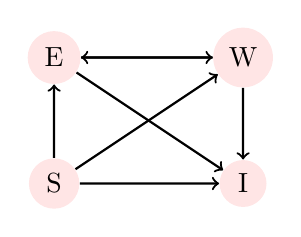
\begin{tikzpicture}
  [scale=.8,auto=left,every node/.style={circle,fill=red!10}]
  \node (n1) at (1,7) {S};
  \node (n2) at (1,9)  {E};
  \node (n3) at (4,9)  {W};
  \node (n4) at (4,7) {I};
 \path[->, draw,thick] 
         (n1) edge (n2)
         (n1) edge (n3)
         (n1) edge (n4)
        (n2) edge (n4)
        (n2) edge (n3)
        (n3) edge (n2)
        (n3) edge (n4);

\end{tikzpicture}
\caption{A directed graph corresponding to the football (soccer) matches shown in Table~\ref{15t1}, with S representing Scotland, E representing England, W representing Wales, and I representing Ireland}\label{15g33}
\end{center}
\end{figure}

Rishnak said, ``Scotland defeated England with a~3-0 record. The goals for and against are
shown in this table''---Rishnak waved his hands and a new table of data appeared [Table~\ref{14t2}]---``Can you figure out all of the scores of the rest of the five games?''

\begin{table}
\begin{center}
\begin{tabular}{ |p{3cm}||p{1.5cm}||p{1.5cm} || }
 \hline
 \multicolumn{3}{|c|}{Goals} \\
 \hline
 Country Name & For & Against \\
 \hline
 Scotland & 7 & 1 \\
 England  & 2 & 3 \\
 Wales    & 3 & 3 \\
 Ireland  & 1 & 6 \\
 
 \hline
\end{tabular}
\caption{Goals for and against for each team}\label{14t2}
\end{center}
\end{table}

Ajur frowned. He could figure out the scores for England immediately, seeing that England defeated Ireland by a score of~2-0 and came to a~0-0 draw with Wales. He spent many long minutes trying various combinations until he finally found a solution. He said, ``Aha, Scotland defeated Wales by a score of~2-1 and defeated Ireland by a score of~2-0. These matched up with the goals for and against Scotland and England. So then Wales defeated Ireland by a score of~2-1. Here, let me write down the results.'' He drew the scores of the six games in the dirt [Table~\ref{14t3}].

\begin{table}
\begin{center}
\begin{tabular}{ |p{3cm}||p{3cm}||p{1.5cm} || }
 \hline
 \multicolumn{3}{|c|}{Game Scores} \\
 \hline
 Country Name & Country Name &Score\\
 \hline
 Scotland & England & 3-0 \\
 Scotland & Wales   & 2-1 \\
 Scotland & Ireland & 2-0 \\
 England  & Wales   & 0-0 \\
 England  & Ireland & 2-0 \\
 Wales    & Ireland & 2-1 \\
  \hline
\end{tabular}
\caption{Scores of the six football (soccer) games}\label{14t3}
\end{center}
\end{table}

%%%%%%%%%%% maybe expand this to relate it to directed graphs and strongly connected components

Rishnak said, ``Good, Ajur. And you should see if you can relate these data to a directed graph. For now, here is one more new concept. A directed graph is acyclic if there are no directed cycles in the graph. Such a graph is called a \textit{directed acyclic graph} or \textit{DAG} for short. Can you draw one?''

Ajur drew a DAG in the dirt [Figure~\ref{15g5}].

\begin{figure}
\begin{center}
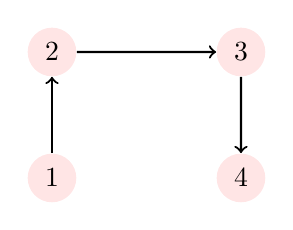
\begin{tikzpicture}
  [scale=.8,auto=left,every node/.style={circle,fill=red!10}]
  \node (n1) at (1,7) {1};
  \node (n2) at (1,9)  {2};
  \node (n3) at (4,9)  {3};
  \node (n4) at (4,7) {4};
 \path[->, draw,thick] 
         (n1) edge (n2)
        (n2) edge (n3)
        (n3) edge (n4);

\end{tikzpicture}
\caption{A directed acyclic graph with four vertices and three edges}\label{15g5}
\end{center}
\end{figure}

Rishnak said, ``A DAG may contain what look like undirected cycles, but it remains a DAG as long as there are no directed cycles.''
Rishnak waved his hands and the graph that Ajur drew appeared in the air. Rishnak said, ``I can add more directed edges''---Rishnak added three more edges [Figure~\ref{15g6}]---``and still this graph is a DAG since it is still acyclic.''

%%Ajur said, ``I see.''

\begin{figure}
\begin{center}
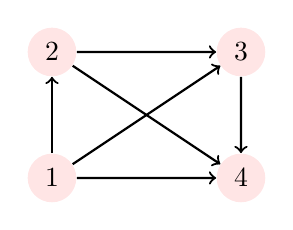
\begin{tikzpicture}
  [scale=.8,auto=left,every node/.style={circle,fill=red!10}]
  \node (n1) at (1,7) {1};
  \node (n2) at (1,9)  {2};
  \node (n3) at (4,9)  {3};
  \node (n4) at (4,7) {4};
 \path[->, draw,thick] 
         (n1) edge (n2)
        (n2) edge (n3)
        (n1) edge (n3)
        (n3) edge (n4)
        (n1) edge (n4)
        (n2) edge (n4);

\end{tikzpicture}
\caption{Another directed acyclic graph}\label{15g6}
\end{center}
\end{figure}

\subsection*{Question for the thirteenth day}
Rishnak said, ``Let me now ask you the question for the thirteenth day. Can you add one edge to make the directed graph you drew in the dirt [Figure~\ref{15g5}] strongly connected?''

\textit{Before you turn the page, try to come up with an answer of your own!}

\newpage
\subsection*{Answer for the thirteenth day}
Ajur responded immediately, ``Sure, that's easy. We can just add a directed edge from vertex~4 to vertex~1 to make the directed graph strongly connected.''

It was getting dark and Jura and Ajur wanted to finish their stroll. Rishnak bade them good night.
